% Created 2020-11-03 mar 15:43
% Intended LaTeX compiler: pdflatex
\documentclass[xcolor={usenames,svgnames,dvipsnames}]{beamer}
\usepackage[utf8]{inputenc}
\usepackage[T1]{fontenc}
\usepackage{graphicx}
\usepackage{grffile}
\usepackage{longtable}
\usepackage{wrapfig}
\usepackage{rotating}
\usepackage[normalem]{ulem}
\usepackage{amsmath}
\usepackage{textcomp}
\usepackage{amssymb}
\usepackage{capt-of}
\usepackage{hyperref}
\usepackage{color}
\usepackage{listings}
\usepackage{mathpazo}
\usepackage{gensymb}
\usepackage{amsmath}
\usepackage{diffcoeff}
\usepackage{steinmetz}
\usepackage{mathtools}
\bibliographystyle{plain}
\usepackage[emulate=units]{siunitx}
\sisetup{fraction=nice, decimalsymbol=comma, retain-unity-mantissa = false}
\newunit{\wattpeak}{Wp}
\newunit{\watthour}{Wh}
\newunit{\amperehour}{Ah}
\hypersetup{colorlinks=true, linkcolor=Blue, urlcolor=Blue}
\renewcommand{\thefootnote}{\fnsymbol{footnote}}
\newcommand{\laplace}[1]{\mathbf{#1}(\mathbf{s})}
\newcommand{\slp}{\mathbf{s}}
\newcommand{\fasor}[1]{\mathbf{#1}(\omega)}
\newcommand{\atan}{\mathrm{atan}}
\parskip=5pt
\usetheme{Boadilla}
\usecolortheme{rose}
\usefonttheme{serif}
\author{Oscar Perpiñán Lamigueiro}
\date{}
\title{Introducción al Régimen Transitorio}
\subtitle{Teoría de Circuitos}
\setbeamercolor{alerted text}{fg=blue!50!black} \setbeamerfont{alerted text}{series=\bfseries}
\AtBeginSubsection[]{\begin{frame}[plain]\tableofcontents[currentsubsection,sectionstyle=show/shaded,subsectionstyle=show/shaded/hide]\end{frame}}
\AtBeginSection[]{\begin{frame}[plain]\tableofcontents[currentsection,hideallsubsections]\end{frame}}
\beamertemplatenavigationsymbolsempty
\setbeamertemplate{footline}[frame number]
\setbeamertemplate{itemize items}[triangle]
\setbeamertemplate{enumerate items}[circle]
\setbeamertemplate{section in toc}[circle]
\setbeamertemplate{subsection in toc}[circle]
\hypersetup{
 pdfauthor={Oscar Perpiñán Lamigueiro},
 pdftitle={Introducción al Régimen Transitorio},
 pdfkeywords={},
 pdfsubject={},
 pdfcreator={Emacs 26.3 (Org mode 9.4)}, 
 pdflang={Spanish}}
\begin{document}

\maketitle

\section{Conceptos Fundamentales}
\label{sec:orgc7a0ee4}

\subsection{¿Qué es el régimen transitorio?}
\label{sec:orge32a169}
\begin{frame}[label={sec:orga6f21ac}]{Permanente y Transitorio}
\begin{block}{Régimen permanente o estacionario}
Las tensiones y corrientes de un circuito son constantes (continua) o periódicas (alterna) (circuito estabilizado)
\end{block}
\begin{block}{Régimen transitorio}
\begin{itemize}
\item Para alcanzar el régimen permanente (o para alternar entre dos regímenes permanentes) el circuito atraviesa el régimen transitorio.
\item Posibles cambios: activación o apagado de fuentes, cambio en las cargas, cambio en el circuito (línea).
\item En general, el estado transitorio es indeseado en sistemas eléctricos, pero provocado en sistemas electrónicos.
\end{itemize}
\end{block}
\end{frame}

\begin{frame}[label={sec:org6e9795f}]{Acumulación de Energía}
\begin{block}{Régimen Permanente}
\alert{Energía acumulada} en \alert{bobinas} y \alert{condensadores}
\end{block}
\begin{block}{Régimen Transitorio}
\begin{itemize}
\item \alert{Redistribución} y \alert{disipación} de energía acumulada.
\item La redistribución de energía \alert{no} se puede realizar de forma \alert{inmediata}
\item \alert{Duración corta} (\(\si{\micro\second}\)) pero superior a 0, dependiendo de \alert{relación entre acumulación y disipación} (resistencia).
\end{itemize}
\end{block}
\end{frame}

\subsection{Condiciones iniciales}
\label{sec:orgd2664fc}
\begin{frame}[label={sec:org75d68c3}]{Respuesta completa de una red lineal}
La respuesta completa de una red lineal a un cambio tiene dos componentes:
\begin{itemize}
\item Respuesta \alert{natural} o propia (sin fuentes, determinada únicamente por la configuración del circuito)
\item Respuesta \alert{forzada} o particular (determinada por las fuentes existentes, \(t = \infty\)).
\end{itemize}
\[
 \boxed{f(t) = f_n(t) + f_\infty(t) }
 \]
\end{frame}

\begin{frame}[label={sec:org94ab19e}]{Condiciones iniciales}
\begin{itemize}
\item Las \alert{condiciones iniciales} son el estado del circuito en el instante temporal en el que se produce el cambio.

\item Determinan las constantes de integración de la respuesta natural.

\item El instante del cambio se representa habitualmente con \(t = 0\):
\begin{itemize}
\item \(t = 0^-\): la topología del circuito es la anterior al cambio.
\item \(t = 0^+\): la topología del circuito es la posterior al cambio.
\end{itemize}
\end{itemize}
\end{frame}
\begin{frame}[label={sec:org36babcc}]{Resistencia}
\[
u(t) = R i(t)
\]

No acumula energía: sigue los cambios de forma instantánea.
\end{frame}

\begin{frame}[label={sec:org6b241ed}]{Inductancia}
\[
u(t) = L \diff{i_L(t)}{t}
\leftrightarrow
i_L(t) = \frac{1}{L} \int^t_{-\infty}u(t') \mathrm{d}t'
\]

La corriente en una bobina no puede variar de forma abrupta (implica tensión infinita).
\[
\boxed{i_L(0^-) = i_L(0^+)}
\]
\end{frame}

\begin{frame}[label={sec:org2694a70}]{Capacidad}
\[
i(t) = C \diff{u_C(t)}{t}
\leftrightarrow
u(t) = \frac{1}{C} \int^t_{-\infty}i(t') \mathrm{d}t'
\]

La tensión en un condensador no puede variar de forma abrupta (implica corriente infinita).
\[
\boxed{u_C(0^-) = u_C(0^+)}
\]
\end{frame}
\begin{frame}[label={sec:org631fae7}]{Ejemplo}
El interruptor lleva en la posición (1) desde un tiempo infinito y  pasa a la posición (2) en \(t = 0\):

\begin{center}
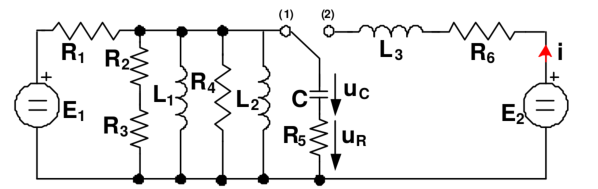
\includegraphics[width=.9\linewidth]{figs/ejemplo_condiciones_iniciales.pdf}
\end{center}
\end{frame}


\section{Circuitos de Primer Orden}
\label{sec:org5771861}
\begin{frame}[label={sec:orgc886cfd}]{Definición}
\begin{itemize}
\item Circuitos que tienen un \alert{único elemento de acumulación} (o \emph{varios elementos que pueden ser simplificados a un elemento equivalente}) y parte resistiva.
\item \alert{Ecuación diferencial de primer orden}: la respuesta natural es siempre una \alert{exponencial decreciente}.
\item Circuitos típicos:
\begin{itemize}
\item RL serie
\item RC paralelo
\end{itemize}
\end{itemize}
\end{frame}
\begin{frame}[label={sec:org10d346b}]{Respuesta natural y forzada}
\begin{itemize}
\item El método de resolución analiza el circuito en dos etapas:
\begin{itemize}
\item Sin fuentes: \alert{respuesta natural} (la energía acumulada en \(t < 0\) se disipa en la resistencia).
\item Con fuentes: \alert{respuesta forzada} (determinada por la forma de onda de las fuentes).
\end{itemize}
\end{itemize}
\end{frame}

\subsection{Circuito RL serie}
\label{sec:orge0f7000}

\begin{frame}[label={sec:orge2c0fd3}]{Circuito básico}
\begin{itemize}
\item En \(t < 0\) la fuente alimenta el circuito RL (la bobina almacena energía).
\item En \(t = 0\) la fuente se desconecta.
\item En \(t > 0\) la bobina se descarga en la resistencia.
\end{itemize}
\begin{center}
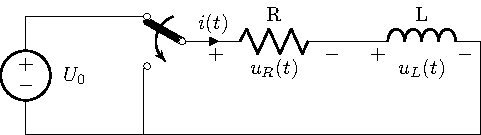
\includegraphics[width=.9\linewidth]{figs/transitorio_circuitoRL.pdf}
\end{center}
\end{frame}

\begin{frame}[label={sec:org684421d}]{Respuesta natural}
\begin{center}
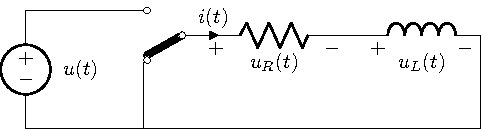
\includegraphics[width=.9\linewidth]{figs/transitorio_circuitoRL_t0+.pdf}
\end{center}
Ecuaciones
\begin{align*}
  u_R(t) + u_L(t) &= 0\\
  R i + L\diff{i}{t} &= 0
\end{align*}

Solución Genérica
\[
  i(t) = A e^{st}
\]
Ecuación Característica
\[
  s + \frac{R}{L} = 0 \Rightarrow s = -\frac{R}{L}
\]
\end{frame}

\begin{frame}[label={sec:orgde5259c}]{Condiciones Iniciales}
Analizando circuito para \(t < 0\) \ldots{} 
\begin{center}
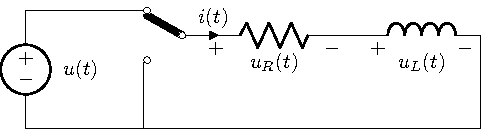
\includegraphics[width=.9\linewidth]{figs/transitorio_circuitoRL_t0-.pdf}
\end{center}
\ldots{}obtenemos  \(i(0^-) = I_0 = \frac{U_0}{R}\) 
\end{frame}

\begin{frame}[label={sec:orgdd8f394}]{Condiciones Iniciales}
Por otra parte, para \(t > 0\):
\begin{align*}
  i(t) &= A e^{-R/L t}\\
  i(0^+) &= A e^0 = A\\
\end{align*}

Y dada la condición de continuidad, \(i(0^+) = i(0^-)\):
\[
  A = I_0
\]
Por tanto, la respuesta natural es:
\[
  \boxed{i(t) = I_0 e^{-R/L t}}
\]
\end{frame}



\begin{frame}[label={sec:orgfa58142}]{Constante de tiempo}
\[
  \boxed{i(t) = I_0 e^{-t/\tau}}
\]

\begin{itemize}
\item \(\tau = \frac{L}{R}\) es la constante de tiempo (unidades [s]).
\item Ratio entre almacenamiento (\(L\)) y disipación (\(R\)).
\item Valores altos de \(\tau\) implican decrecimiento lento.
\item La respuesta natural \guillemotleft{}desaparece\guillemotright{} tras \(\simeq 5\tau\).
\end{itemize}
\begin{center}
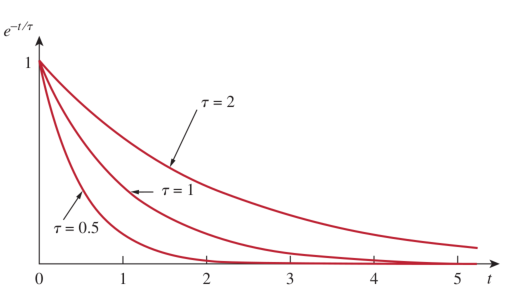
\includegraphics[height=0.5\textheight]{figs/constante_tiempo.pdf}
\end{center}
\end{frame}

\begin{frame}[label={sec:orgd0ee3e7}]{Balance Energético}
La energía acumulada en la bobina en \(t < 0\) se disipa en la resistencia en \(t > 0\)

\begin{align*}
  W_R &= \int_0^\infty R i^2(t)  \mathrm{d}t =\\
  &= \int_0^\infty R (I_0 e^{-t/\tau})^2  \mathrm{d}t = \\
  &= \frac{1}{2} L I_0^2 = W_L  
\end{align*}
\end{frame}

\begin{frame}[label={sec:org505b081}]{Respuesta forzada}
Cambiemos el funcionamiento del interruptor: en \(t > 0\) la fuente alimenta el circuito RL.
\begin{center}
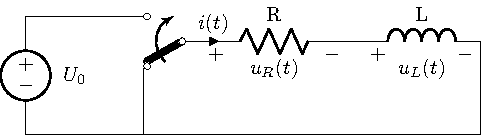
\includegraphics[width=.9\linewidth]{figs/transitorio_circuitoRL2.pdf}
\end{center}
\end{frame}

\begin{frame}[label={sec:org2e81179}]{Respuesta forzada}
\begin{center}
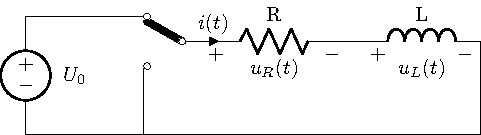
\includegraphics[width=.9\linewidth]{figs/transitorio_circuitoRL2_t0+.pdf}
\end{center}
Las ecuaciones son ahora:
\[
  u_R(t) + u_L(t) = u(t) \rightarrow R i + L\diff{i}{t} = U_0
\]

Para la solución particular, \(i_\infty\), se propone una función análoga a la excitación (analizando circuito para \(t > 0\))
\begin{align*}
  i(t) &= i_n(t) + i_\infty(t)\\
  i_n(t) &= A e^{st}\\
  i_\infty(t) &= U_0/R\\
\end{align*}
\end{frame}

\begin{frame}[label={sec:org06e5dbc}]{Condiciones iniciales}
Particularizamos las ecuaciones en \(t = 0^+\):
\begin{align*}
  i(0^+) &= i_n(0^+) + i_\infty(0^+)\\
  i(0^+) &= A + i_\infty(0^+)\\
  A &= i(0^+) - i_\infty(0^+)
\end{align*}
\end{frame}

\begin{frame}[label={sec:org516cf4f}]{Respuesta completa (ejemplo)}
\begin{align*}
  i(t) &= i_n(t) + i_\infty(t)\\
  i_n(t) &= A e^{st}\\
  i_\infty(t) &= U_0/R\\
  A &= i(0^+) - i_\infty(0^+)
\end{align*}

Suponiendo que la bobina está inicialmente descargada, \(i(0^-) = 0\), y teniendo en cuenta la condición de continuidad, \(i(0^+) = i(0^-) = 0\), obtenemos \(A= 0 - U_0/R\). 

La solución completa es:
\[
  \boxed{i(t) = \frac{U_0}{R}(1 - e^{-\frac{t}{\tau}})  }
\]
\end{frame}

\begin{frame}[label={sec:org22fbc6b}]{Respuesta completa}
\[
  \boxed{i(t) = \frac{U_0}{R}(1 - e^{-\frac{t}{\tau}})  }
\]

\begin{center}
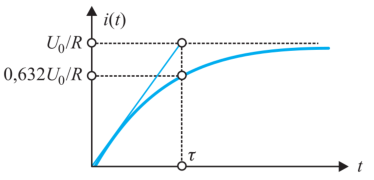
\includegraphics[width=.9\linewidth]{figs/RespuestaCompleta_RL.pdf}
\end{center}
\end{frame}


\begin{frame}[label={sec:orgcceea15}]{Expresión general de la respuesta completa}
\[
\boxed{i(t) = \left[i(0^+) - i_\infty(0^+)\right] e^{-t/\tau} + i_\infty(t)}
\]

\begin{itemize}
\item \(i(0^+)\): corriente en la bobina, condiciones iniciales, \(i(0^-) = i(0^+)\).
\item \(i_\infty(t)\): corriente en la bobina en régimen permanente para \(t > 0\).
\item \(i_\infty(0^+)\): corriente en la bobina en régimen permanente particularizada en \(t = 0\).
\end{itemize}
\end{frame}

\begin{frame}[label={sec:orgf35fb15}]{Equivalente de Thévenin}
\begin{center}
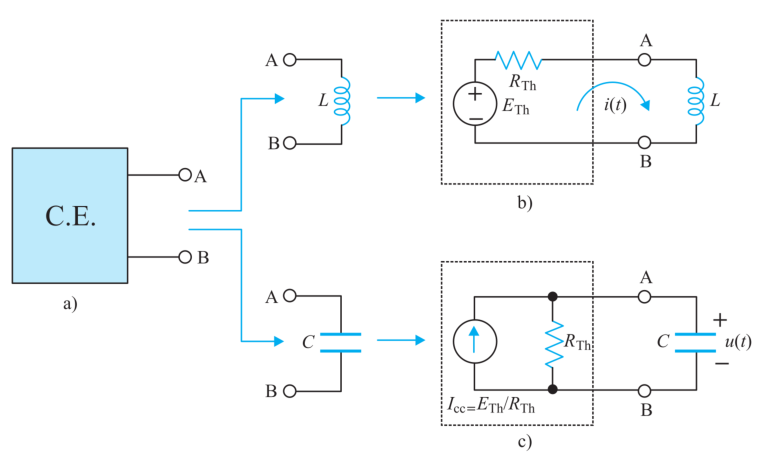
\includegraphics[width=.9\linewidth]{figs/Thevenin_PrimerOrden.pdf}
\end{center}
\end{frame}
\subsection{Circuito RC paralelo}
\label{sec:org5b7da04}

\begin{frame}[label={sec:org4c2211d}]{Circuito básico}
\begin{itemize}
\item En \(t <0\) la fuente alimenta el circuito RC (el condensador se carga).
\item En \(t = 0\) se desconecta la fuente (el condensador comienza a descargarse en la resistencia).
\end{itemize}
\begin{center}
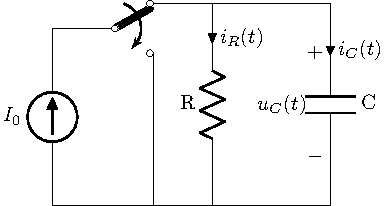
\includegraphics[width=.9\linewidth]{figs/transitorio_circuitoRC.pdf}
\end{center}
\end{frame}

\begin{frame}[label={sec:org7189046}]{Respuesta natural}
\begin{center}
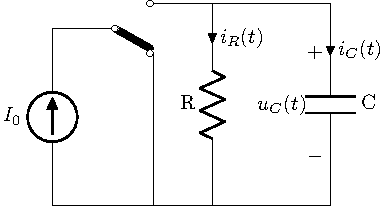
\includegraphics[height=0.3\textheight]{figs/transitorio_circuitoRC_t0+.pdf}
\end{center}

Ecuaciones
\begin{align*}
  i_R(t) + i_C(t) &= 0\\
  G u + C\diff{u}{t} &= 0
\end{align*}

Solución Genérica
\[
  u(t) = A e^{st}
\]

Respuesta natural
\[
  \boxed{u(t) = U_0 e^{-G/C t}}
\]
\end{frame}



\begin{frame}[label={sec:orgaec2210}]{Constante de tiempo}
\begin{itemize}
\item \(\tau = \frac{C}{G}\) es la constante de tiempo (unidades [s]).
\item Ratio entre almacenamiento (\(C\)) y disipación (\(G\)).
\end{itemize}

\[
  \boxed{u(t) = U_0 e^{-t/\tau}  }
\]

\begin{center}
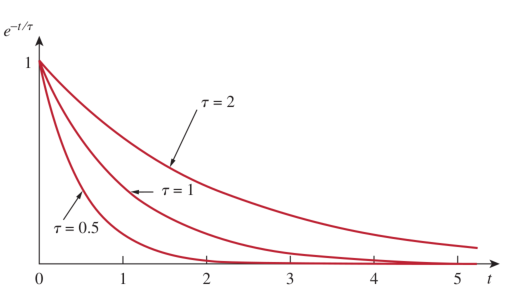
\includegraphics[width=.9\linewidth]{figs/constante_tiempo.pdf}
\end{center}
\end{frame}

\begin{frame}[label={sec:orgdaa3144}]{Balance Energético}
La energía acumulada en el condensador en \(t < 0\) se disipa en la resistencia (conductancia) en \(t > 0\)

\[
  W_G = \int_0^\infty G u^2(t)  \mathrm{d}t = \frac{1}{2} C U_0^2 = W_C
\]
\end{frame}

\begin{frame}[label={sec:org0493fc8}]{Expresión general de la respuesta completa}
\[
\boxed{u(t) = \left[u(0^+) - u_\infty(0^+)\right] e^{-t/\tau} + u_\infty(t)}
\]

\begin{itemize}
\item \(u(0^+)\): tensión en el condensador, condiciones iniciales, \(u(0^-) = u(0^+)\).
\item \(u_\infty(t)\): tensión en el condensador en régimen permanente para \(t > 0\).
\item \(u_\infty(0^+)\): tensión en el condensador en régimen permanente particularizada en \(t = 0\).
\end{itemize}
\end{frame}

\begin{frame}[label={sec:org815fcb1}]{Ejemplo con respuesta forzada}
\begin{center}
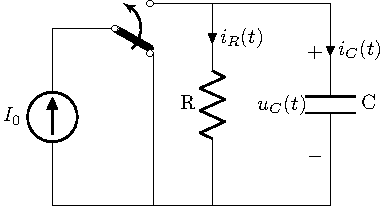
\includegraphics[height=0.3\textheight]{figs/transitorio_circuitoRC2.pdf}
\end{center}

\[
\boxed{u(t) = \left[u(0^+) - u_\infty(0^+)\right] e^{-t/\tau} + u_\infty(t)}
\]

Suponiendo que el condensador está inicialmente descargado:
\begin{align*}
  u(0^+) &= u(0^-) = 0\\
  u_\infty(0^+) &= I_0/G\\
  u(t) &= \frac{I_0}{G}(1 - e^{-\frac{t}{\tau}})  
\end{align*}
\end{frame}

\begin{frame}[label={sec:org2e8f1ff}]{Equivalente de Norton}
\begin{center}
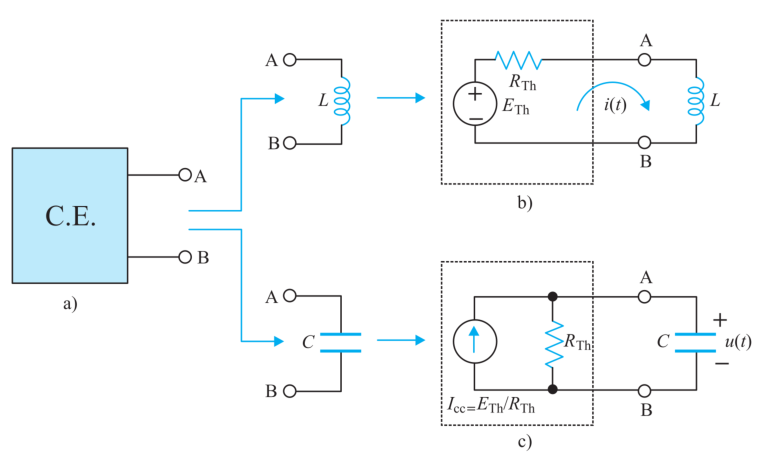
\includegraphics[width=.9\linewidth]{figs/Thevenin_PrimerOrden.pdf}
\end{center}
\end{frame}

\subsection{Análisis Sistemático}
\label{sec:org8b3e8fc}

\begin{frame}[label={sec:orgdfce418}]{Equivalente de Thévenin/Norton}
\begin{center}
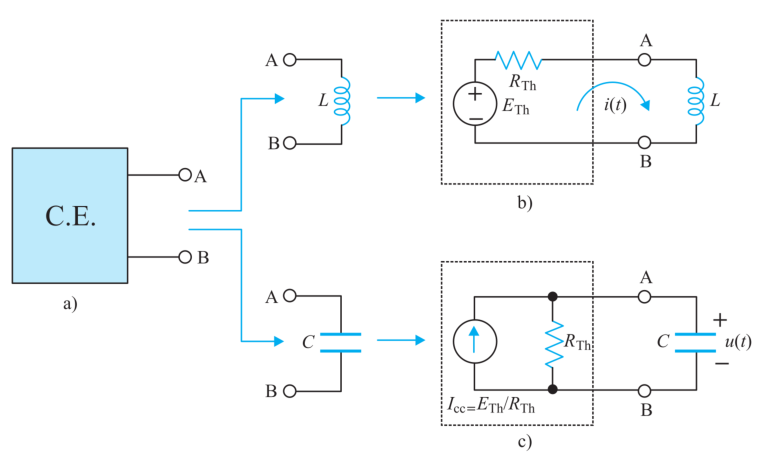
\includegraphics[width=.9\linewidth]{figs/Thevenin_PrimerOrden.pdf}
\end{center}
\end{frame}

\begin{frame}[label={sec:orgd48148f}]{Procedimiento General}
\begin{itemize}
\item Dibujar el circuito para \(t < 0\).
\begin{itemize}
\item Determinar variables en régimen permanente, \(u_c(t)\), \(i_L(t)\).
\item Particularizar para \(t = 0\), obteniendo \(u_c(0^-)\) o \(i_L(0^-)\).
\item Continuidad: \(u_c(0^+) = u_c(0^-)\), \(i_L(0^+) = i_L(0^-)\).
\end{itemize}
\item Dibujar el circuito para \(t > 0\).
\begin{itemize}
\item Calcular el equivalente de Thevenin (Norton) visto por el elemento de acumulación.
\item La constante de tiempo de la respuesta natural es \(\tau = \frac{L}{R_{th}}\) o \(\tau = \frac{C}{G_{th}}\).
\item Calcular las variables \(i_L(t)\) o \(u_c(t)\) en régimen permanente, obteniendo \(i_\infty(t)\) o \(u_\infty(t)\).
\end{itemize}
\item Obtener respuesta completa:
\end{itemize}
\begin{align*}
i_L(t) &= \left(i_L(0^+) - i_\infty(0^+)\right) e^{-t/\tau} + i_\infty(t)\\
u_C(t) &= \left(u_C(0^+) - u_\infty(0^+)\right) e^{-t/\tau} + u_\infty(t)\\
\end{align*}
\end{frame}


\section{Circuitos de Segundo Orden}
\label{sec:org6444b4b}
\begin{frame}[label={sec:orgb03ec7a}]{Introducción}
\begin{itemize}
\item Circuitos que tienen \alert{dos elementos de acumulación} que intercambian energía, y parte resistiva que disipa energía.
\item \alert{Ecuación diferencial de segundo orden}: la respuesta natural incluye exponenciales decrecientes y quizás señal sinusoidal.
\item Circuitos típicos:
\begin{itemize}
\item RLC serie
\item RLC paralelo
\end{itemize}
\end{itemize}
\end{frame}
\begin{frame}[label={sec:org0fd2c84}]{Respuesta natural y forzada}
\begin{itemize}
\item El método de resolución analiza el circuito en dos etapas:
\begin{itemize}
\item Sin fuentes: \alert{respuesta natural} (la energía acumulada en \(t < 0\) se redistribuye).
\item Con fuentes: \alert{respuesta forzada} (determinada por la forma de onda de las fuentes).
\end{itemize}
\end{itemize}
\end{frame}

\subsection{Circuito RLC serie}
\label{sec:orgfc6a40c}
\begin{frame}[label={sec:org650ea99}]{Circuito básico}
\begin{center}
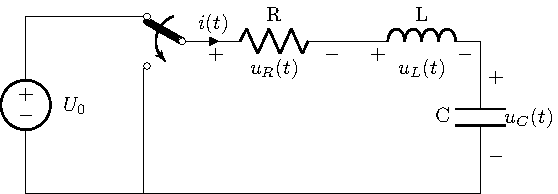
\includegraphics[width=.9\linewidth]{figs/transitorio_circuitoRLC_serie.pdf}
\end{center}
\end{frame}


\begin{frame}[label={sec:org3e1aa0d}]{Respuesta natural (t > 0)}
\begin{center}
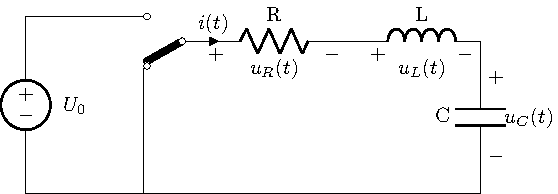
\includegraphics[width=.9\linewidth]{figs/transitorio_circuitoRLC_serie_t0+.pdf}
\end{center}

\[
  Ri(t) + L\diff{i(t)}{t} + \frac{1}{C}\int_{-\infty}^t i(t') \mathrm{d}t' = 0
\]

\[
  L\diff[2]{i}{t} + R\diff{i}{t} + \frac{1}{C} i = 0 \Rightarrow
  \boxed{\diff[2]{i}{t} + \frac{R}{L} \diff{i}{t} + \frac{1}{LC} i = 0}
\]
\end{frame}

\begin{frame}[label={sec:org69520d8}]{Solución}
\begin{block}{Ecuación diferencial}
\[
\diff[2]{i}{t} + \frac{R}{L} \diff{i}{t} + \frac{1}{LC} i = 0
\]
\[
    i_n(t) = A_1 e^{s_1 t} + A_2 e^{s_2 t}
\]
\end{block}

\begin{block}{Ecuación característica}
\[
s^2 + \frac{R}{L} s + \frac{1}{LC} = 0  
\]
\[
  s_{1,2} = -\frac{R}{2L} \pm \sqrt{\left(\frac{R}{2L}\right)^2 - \frac{1}{LC}}
\]
\end{block}
\end{frame}


\begin{frame}[label={sec:orgd5b2cbf}]{Parámetros}
\begin{columns}
\begin{column}{.5\columnwidth}
\begin{align*}
  s^2 + \frac{R}{L} s + \frac{1}{LC} &= 0\\
  s^2 + 2\alpha s + \omega_0^2 &= 0  
\end{align*}

\[
  s_{1,2} = -\alpha \pm \sqrt{\alpha^2 - \omega_0^2}
\]
\[
  i_n(t) = A_1 e^{s_1 t} + A_2 e^{s_2 t}
\]
\end{column}

\begin{column}{.5\columnwidth}
\begin{align*}
  \alpha &= \frac{R}{2L}\\
  \omega_0 &= \frac{1}{\sqrt{LC}}\\
  \omega_d &= \sqrt{\omega_0^2 - \alpha^2}\\
  \xi &= \frac{\alpha}{\omega_0}
\end{align*}
\end{column}
\end{columns}
\vspace{1cm}
\begin{itemize}
\item \(\alpha\): coeficiente de amortiguamiento exponencial
\item \(\omega_0\): pulsación natural no amortiguada
\item \(\omega_d\): pulsación natural amortiguada
\item \(\xi\): factor de amortiguamiento
\end{itemize}
\end{frame}
\begin{frame}[label={sec:org4558d9c}]{Posibles soluciones}
\[
  \boxed{s_{1,2} = -\alpha \pm \sqrt{\alpha^2 - \omega_0^2}}
\]

\begin{block}{\(\alpha > \omega_0\), \(\xi > 1\)}
\begin{itemize}
\item \(s_{1,2}\): dos soluciones reales (negativas) distintas
\item Circuito \alert{sobreamortiguado}.
\end{itemize}
\end{block}

\begin{block}{\(\alpha = \omega_0\), \(\xi = 1\)}
\begin{itemize}
\item \(s_{1,2}\): solución real doble.
\item Circuito con \alert{amortiguamiento crítico}.
\end{itemize}
\end{block}

\begin{block}{\(\alpha < \omega_0\), \(\xi < 1\)}
\begin{itemize}
\item \(s_{1,2}\): dos soluciones complejas conjugadas
\item Circuito \alert{subamortiguado}.
\end{itemize}
\end{block}
\end{frame}

\begin{frame}[label={sec:orge8200d4}]{Tipos de Respuesta}
\begin{itemize}
\item Tipo de respuesta determinado por relación entre \(R\) y \(L\), \(C\) (disipación y almacenamiento).
\item Resistencia crítica (\(\alpha = \omega_0\), \(\xi = 1\)):
\end{itemize}

\[
  R_{cr} = 2\sqrt{\frac{L}{C}}
\]

\begin{block}{Tipos}
\begin{itemize}
\item \(R > R_{cr}\), \(\alpha > \omega\), \(\xi > 1\): \alert{sobreamortiguado}
\item \(R = R_{cr}\),  \(\alpha = \omega\), \(\xi = 1\): \alert{amortiguamiento crítico}
\item \(R < R_{cr}\),  \(\alpha < \omega\), \(\xi < 1\): \alert{subamortiguado}
\end{itemize}
\end{block}
\end{frame}

\begin{frame}[label={sec:orgfd52a99}]{Circuito Sobreamortiguado (\(\alpha > \omega_0\))}
\[
  \boxed{i_n(t) = A_1 e^{s_1 t} + A_2 e^{s_2 t}}
\]

\begin{center}
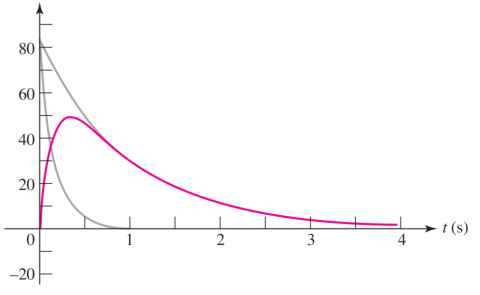
\includegraphics[width=.9\linewidth]{figs/Sobreamortiguado_HKD.pdf}
\end{center}
\end{frame}

\begin{frame}[label={sec:org562675b}]{Amortiguamiento Crítico (\(\alpha = \omega_0\))}
\[
  \boxed{i_n(t) = (A_1 + A_2 t) e^{s t} }
\]

\begin{center}
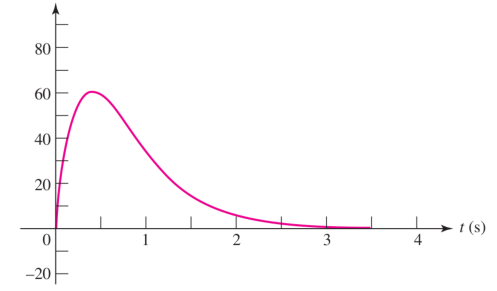
\includegraphics[width=.9\linewidth]{figs/AmortiguamientoCritico_HKD.pdf}
\end{center}
\end{frame}


\begin{frame}[label={sec:orgba11872}]{Circuito Subamortiguado (\(\alpha < \omega\))}
\[
  \boxed{i_n(t) = (B_1\cos(\omega_d t) + B_2\sin(\omega_d t)) e^{-\alpha t}}
\]

\begin{center}
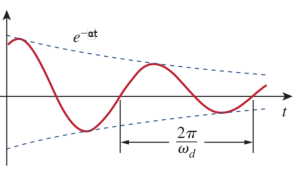
\includegraphics[width=.9\linewidth]{figs/Subamortiguado_AS.pdf}
\end{center}
\end{frame}

\begin{frame}[label={sec:org0f9899c}]{Valores Importantes}
\begin{center}
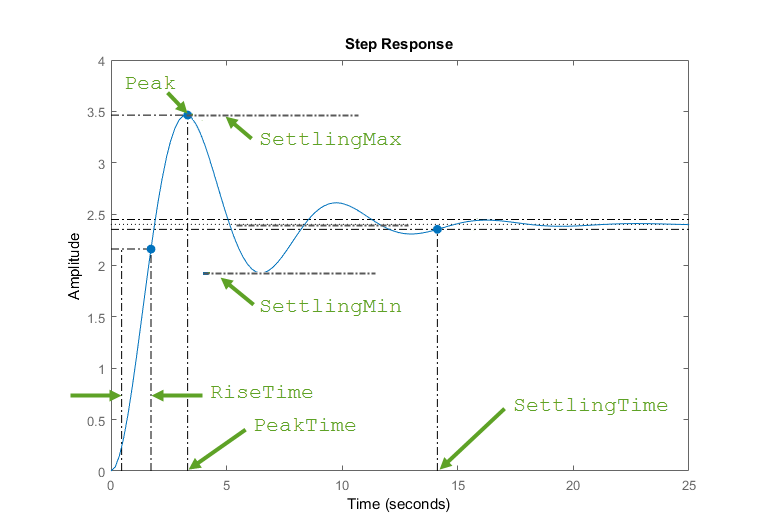
\includegraphics[height=0.6\textheight]{figs/RespuestaEscalon_SegundoOrden.png}
\end{center}

\begin{itemize}
\item \alert{Tiempo de Subida}: tiempo para subir de 10\% al 90\% del valor en régimen permanente.

\item \alert{Tiempo de Establecimiento}: tiempo para que la diferencia entre la respuesta y el régimen permanente permanezca dentro de una banda del 1\%.
\end{itemize}
\end{frame}

\begin{frame}[label={sec:org6149c88}]{Valores Importantes}
\begin{center}
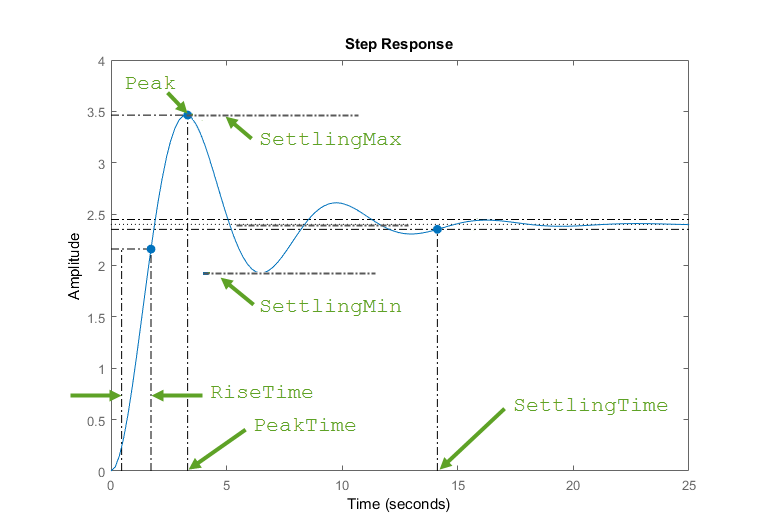
\includegraphics[height=0.6\textheight]{figs/RespuestaEscalon_SegundoOrden.png}
\end{center}

\begin{itemize}
\item \alert{Valor máximo} y \alert{Tiempo del Valor Máximo}.

\item \alert{Sobretensión}: porcentaje del valor máximo respecto del régimen permanente.
\end{itemize}
\end{frame}


\begin{frame}[label={sec:org02d2dc9}]{Condiciones Iniciales}
\begin{block}{Dos constantes a determinar}
Son necesarias dos tipos de condiciones iniciales:

\begin{align*}
  i_L(0^+) &= i_L(0^-)\\
  u_L(t) = L \cdot \diff{i_L(t)}{t} \longrightarrow   \diff{i_L(t)}{t}{t = 0^+} &= \frac{1}{L} u_L(0^+)
\end{align*}
\end{block}

\begin{block}{Derivadas en el origen}
Para obtener valores de las derivadas en el origen hay que resolver el circuito en \(t = 0^+\) empleando las condiciones de continuidad.
\end{block}
\end{frame}

\begin{frame}[label={sec:org426db32}]{Derivadas en \(t = 0^+\)}
\begin{center}
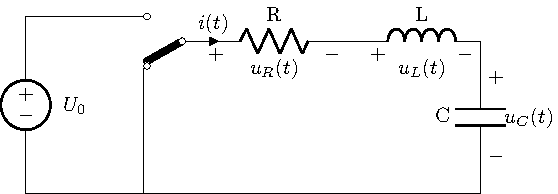
\includegraphics[height=0.35\textheight]{figs/transitorio_circuitoRLC_serie_t0+.pdf}
\end{center}

\[
  \diff{i_L(t)}{t}{t = 0^+} = \frac{1}{L} u_L(0^+)
\]
\begin{align*}
  u_L(0^+) &= -u_R(0^+) - u_c(0^+)\\
  u_R(0^+) &= R i_L(0^+)
\end{align*}
\[
\boxed{\diff{i_L(t)}{t}{t = 0^+} = - \frac{1}{L}\left(R i_L(0^+) + u_c(0^+)\right)}
\]
\end{frame}

\begin{frame}[label={sec:orgcd2cba9}]{Respuesta Completa}
Las condiciones iniciales deben evaluarse teniendo en cuenta la respuesta forzada (si existe).
\begin{align*}
  i_L(0^+) &= i_n(0^+) + i_{\infty}(0^+)\\
  \diff{i_L}{t}{t = 0^+} &= \diff{i_n}{t}{t = 0^+} + \diff{i_{\infty}}{t}{t = 0^+}  
\end{align*}
\end{frame}

\begin{frame}[label={sec:org2e9402d}]{Ejemplo de Respuesta Completa}
Circuito RLC serie sobreamortiguado con generador de tensión DC funcionando en \(t > 0\). 

\begin{block}{Respuesta Completa}
\[
  i_L(t) = I_{\infty} + A_1 e^{s_1 t} + A_2 e^{s_2 t}
\]
\end{block}

\begin{block}{Condiciones Iniciales}
\begin{align*}
i_L(0^+) &= I_\infty + A_1 + A_2\\
\diff{i_L(t)}{t}{t = 0^+} &= 0 + A_1 s_1 + A_2 s_2
\end{align*}
\end{block}
\end{frame}


\subsection{Circuito RLC paralelo}
\label{sec:org58b3aa9}
\begin{frame}[label={sec:org68e52a0}]{Circuito básico}
\begin{center}
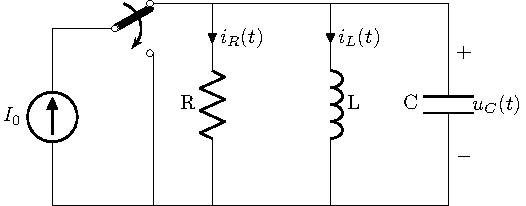
\includegraphics[width=.9\linewidth]{figs/transitorio_circuitoRLC_paralelo.pdf}
\end{center}
\end{frame}

\begin{frame}[label={sec:orgf58f6b8}]{Respuesta natural (t > 0)}
\begin{center}
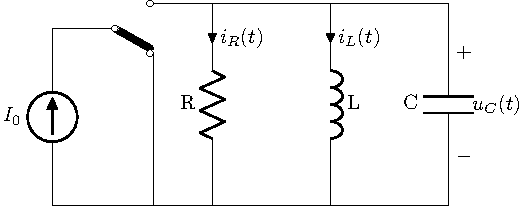
\includegraphics[width=.9\linewidth]{figs/transitorio_circuitoRLC_paralelo_t0+.pdf}
\end{center}

\[
  Gu(t) + C\diff{u(t)}{t} + \frac{1}{L}\int_{-\infty}^t u(t') \mathrm{d}t' = 0
\]

\[
  \diff[2]{u}{t} + \frac{G}{C} \diff{u}{t} + \frac{1}{LC} u = 0
\]
\end{frame}

\begin{frame}[label={sec:orgc286047}]{Solución}
\begin{block}{Ecuación diferencial}
\[
  \diff[2]{u}{t} + \frac{G}{C} \diff{u}{t} + \frac{1}{LC} u = 0
\]
\[
  u_n(t) = A_1 e^{s_1 t} + A_2 e^{s_2 t}
\]
\end{block}

\begin{block}{Ecuación característica}
\[
s^2 + \frac{G}{C} s + \frac{1}{LC} = 0  
\]
\[
  s_{1,2} = -\frac{G}{2C} \pm \sqrt{\left(\frac{G}{2C}\right)^2 - \frac{1}{LC}}
\]
\end{block}
\end{frame}


\begin{frame}[label={sec:org4cc3100}]{Parámetros}
\begin{block}{Ecuación característica}
\begin{columns}
\begin{column}{.5\columnwidth}
\begin{align*}
s^2 + \frac{G}{C} s + \frac{1}{LC} &= 0\\
s^2 + 2\alpha s + \omega_0^2 &= 0  
\end{align*}

\[
  s_{1,2} = -\alpha \pm \sqrt{\alpha^2 - \omega_0^2}
\]

\[
  u_n(t) = A_1 e^{s_1 t} + A_2 e^{s_2 t}
\]
\end{column}
\begin{column}{.5\columnwidth}
\begin{align*}
  \alpha &= \frac{G}{2C}\\
  \omega_0 &= \frac{1}{\sqrt{LC}}\\
  \omega_d &= \sqrt{\omega_0^2 - \alpha^2}\\
  \xi &= \frac{\alpha}{\omega_0}
\end{align*}
\end{column}
\end{columns}
\end{block}
\end{frame}

\begin{frame}[label={sec:orgc405401}]{Tipos de Respuesta}
\begin{itemize}
\item Tipo de respuesta determinado por relación entre \(G\) y \(L\), \(C\) (disipación y almacenamiento).
\item Conductancia crítica (\(\alpha = \omega_0\), \(\xi = 1\)):
\end{itemize}

\[
  G_{cr} = 2\sqrt{\frac{C}{L}}
\]

\begin{block}{Tipos}
\begin{itemize}
\item \(G > G_{cr}\), \(\alpha > \omega\), \(\xi > 1\): \alert{sobreamortiguado}
\item \(G = G_{cr}\),  \(\alpha = \omega\), \(\xi = 1\): \alert{amortiguamiento crítico}
\item \(G < G_{cr}\),  \(\alpha < \omega\), \(\xi < 1\): \alert{subamortiguado}
\end{itemize}
\end{block}
\end{frame}

\begin{frame}[label={sec:org5ae160a}]{Tipos de Respuesta}
\begin{itemize}
\item Circuito Sobreamortiguado (\(\alpha > \omega_0\))
\end{itemize}
\[
  \boxed{u_n(t) = A_1 e^{s_1 t} + A_2 e^{s_2 t}}
\]
\begin{itemize}
\item Amortiguamiento Crítico (\(\alpha = \omega_0\))
\end{itemize}
\[
  \boxed{u_n(t) = (A_1 + A_2 t) e^{s t} }
\]

\begin{itemize}
\item Circuito Subamortiguado (\(\alpha < \omega\))
\end{itemize}
\[
  \boxed{u_n(t) = (B_1\cos(\omega_d t) + B_2\sin(\omega_d t)) e^{-\alpha t}}
\]
\end{frame}


\begin{frame}[label={sec:org1ede279}]{Condiciones Iniciales}
\begin{block}{Dos constantes a determinar}
Son necesarias dos tipos de condiciones iniciales:


\begin{align*}
  u_C(0^+) &= u_C(0^-)\\
  i_c(t) = C \cdot \diff{u_c(t)}{t} \longrightarrow \diff{u_c(t)}{t}{t = 0^+} &= \frac{1}{C}i_C(0^+)
\end{align*}
\end{block}

\begin{block}{Derivadas en el origen}
Para obtener valores de las derivadas en el origen hay que resolver el circuito en \(t = 0^+\) empleando las condiciones de continuidad.
\end{block}
\end{frame}

\begin{frame}[label={sec:org9065bc3}]{Derivadas en \(t = 0^+\): ejemplo RLC paralelo}
\begin{center}
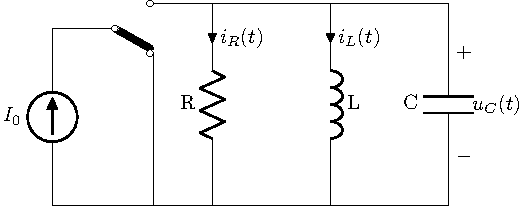
\includegraphics[height=0.35\textheight]{figs/transitorio_circuitoRLC_paralelo_t0+.pdf}
\end{center}

\[
  \diff{u_c(t)}{t}{t = 0^+} = \frac{1}{C}i_C(0^+)
\]

\begin{align*}
  i_C(0^+) &= -i_R(0^+) - i_L(0^+)\\
  i_R(0^+) &= \frac{1}{R} u_C(0^+)
\end{align*}
\[
  \boxed{\diff{u_c(t)}{t}{t = 0^+} = - \frac{1}{C} \left( \frac{1}{R} u_C(0^+) +  i_L(0^+)\right)}
\]
\end{frame}


\begin{frame}[label={sec:orge0f7ab2}]{Respuesta Completa}
Las condiciones iniciales deben evaluarse teniendo en cuenta la respuesta forzada (si existe).
\begin{align*}
  u_C(0^+) &= u_n(0^+) + u_{\infty}(0^+)\\
  \diff{u_C(t)}{t}{t = 0^+} &= \diff{u_n(t)}{t}{t = 0^+} + \diff{u_{\infty}(t)}{t}{t = 0^+}  
\end{align*}
\end{frame}

\begin{frame}[label={sec:org7216e35}]{Ejemplo de Respuesta Completa}
Circuito RLC paralelo sobreamortiguado con generador de corriente DC funcionando en \(t > 0\). 

\begin{block}{Respuesta Completa}
\[
  u_c(t) = U_{\infty} + A_1 e^{s_1 t} + A_2 e^{s_2 t}
\]
\end{block}

\begin{block}{Condiciones Iniciales}
\begin{align*}
u_c(0^+) &= U_\infty + A_1 + A_2\\
\diff{u_C(t)}{t}{t = 0^+} &= 0 + A_1 s_1 + A_2 s_2
\end{align*}
\end{block}
\end{frame}
\end{document}